\chapter{Einleitung}
\label{sec:Einleitung}

\comment{needs Text here}

\section{Motivation}
\label{sec:motivation}
Research into compilers leads to efficient transformation of stuff into other stuff.
The formal definition can be seen in \cref{tab:manualeval}.
Description of results is done in \cref{sec:results} and shown in \cref{fig:searchtree}.

\chapter{i-Core}

\chapter{SHA-3}

\chapter{Implementierung}
\label{sec:first_iteration}

\section{Erste Iteration}
\subsection{Entwurfsziele}

Die Architektur gibt eine maximale Größe von 1600 LUTs für seine Beschleunigerblöcke vor und ein Beschleuniger kann aus maximal 5 solcher Blöcke bestehen.
Weiterhin permutiert die Keccak-Funktion ein 1600 Bit breites Feld, wobei jedes Bit von vielen anderen Bits an verschiedenen Stellen im Feld abhängt.
Da die verschiedenen Blöcke nicht beliebig miteinander kommunizieren können, sondern nur über eine taktsynchrone Schnittstelle mit sehr begrenzter Bandbreite,
folgt aus den beiden Beobachtungen die Vermutung, dass ein guter Beschleuniger aus so wenig Blöcken wie möglich besteht.
Ziel des ersten Entwurfs war daher einen Beschleuniger zu entwickeln, der die Keccak-Permutation so schnel wie möglich in einem Block berechnet.
Dabei war es erlaubt die Größenbeschränkung von 1600 LUTs in einem sinnvollen Maß zu überschreiten um daraufhin das Optimierungspotential des Entwurfs zu untersuchen
und nach und nach die Größe zu reduzieren, bis schließlich das Größenlimit eingehalten wird.
So sollten zum Beispiel nicht einfach alle 24 Runden in einem Takt über eine riesige kombinatorische Schaltung berechnet werden,
da selbst für eine einzelne Runde die 1600 LUTs für die 1600 Bit Ausgabe schon kritisch sind.
Weil sich die einzelnen Runden voneinander nur in einem Rundenindex unterscheiden, der sich in einer 64-Bit Konstanten in der Iota-Funktion manifestiert,
hätte man eine um Größenordnungen zu große Schaltung mit sehr viel repetetiver Logik.

\subsection{Aufbau}
Daher Bestand der erste Entwurf direkt aus einer kombinatorischen Schaltung, die eine komplette Runde berechnet sowie einem Register,
das die Ausgabe dieser Schaltung speichert und wieder als Eingabe bereit stellt.
[Bild hier + Beschreibung]

\subsection{Bewertung}
Letztendlich besteht der erste Entwurf aus \comment{circa 3500 LUTs, Zahl muss noch präzisiert werden} ohne Kommunikationslogik.
Die Zahl setzt sich aus ungefähr 1600 LUTS für das Speichern der Daten zusammen und der Rest wird von der kombinatorischen Rundenfunktion benötigt.
Das ist zwar noch etwa doppelt so groß wie das finale Design am Ende sein soll, aber mit ein paar Anpassungen kann die größe potentiell weiter reduziert werden.

\subsection{Optimierungsansätze}
Der wohl naheliegendste Gedanke ist den Datenspeicher zu reduzieren, da er mit seinen 1600 LUTs bereits das gesammte Budget alleine benötigt.

\subsubsection{Aufspalten der Rundenfunktion}
Um die Rundenfunktion in mehrere Teile aufteilen zu können, ist eine genauere Untersuchung der Funktion selbst notwendig um Teie ausfindig zu machen,
die unabhängig voneinander berechnet werden können. Das Aufteilen in die gleichen Teilfunktionen, aus denen sie zusammengesetzt ist, ist nicht sinnvoll.
Jede einzelne der Funktionen Theta, Rho, Pi und Chi hat genau die gleiche Eingabelänge. Es müssen also auch die Teilfunktionen selbst aufgeteilt werden.

Folgendes lässt sich aber über die einzelnen Teilfunktionen festhalten:
Theta ist eine Slice-orientierte Funktion.
Jeder Slice S(i) der Ausgabe hängt nur von zwei Slices S(i) und S(i - 1) der Eingabe ab.
Rho hingegen ist eine Lane-orientierte Funktion. Genauer genommen einfach ein Bit-Rotate jeder Lane, wobei die Weite der Rotation vom Index der Lane abhängt.
Pi und Chi sind auch Slice-orientiert, anders als Theta hängt jedoch ein Ausgabe-Slice S(i) nur von einem Einzigen Eingabe-Slice S(i) ab.
Iota ist ein Spezialfall; da sie nur eine Rundenkonstante auf eine einzige Lane aufaddiert.
Dieses Operation kann aber auch als Slice-Operation Iota(S(i), i, r) dargestellt werden, die zusätzlich von dem Slice-Index i abhängt.
Jede Teilfunktion lässt sich also Schrittweise mit einem Teil des Datenblocks berechnen, wobei Rho sich in der Hinsicht von den anderen Funktionen unterscheidet,
dass sie Lane-orientiert arbeitet. Die Rundenfunktion Rnd(r) = Iota(r) . Chi . Pi . Rho . Theta kann also in mehrere Schritte unterteilt werden,
die den Datenblock wiederum in jeweils mehreren Schritten verarbeiten. Weiterhin sollen allerdings so viele Teilfunktionen wie möglich
zusammengefasst werden können, um die benötigte Anzahl an Schritten zu minimieren. Durch Abrollen der Permutationsfunktion lässt sich diese Anzahl auf zwei reduzieren.
Rollt man die Permutationsfunktion
einmal ab, so erhält man nach Einsetzen der Definition von $Rnd_r$:
\begin{align*}
    \text{KECCAK-p} & = \bigcomp_{r = 0}^{23} Rnd_r = \bigcomp_{r = 0}^{23} \iota_r \circ \chi \circ \pi \circ \rho \circ \theta \\
    & = \iota_{23} \circ \chi \circ \pi \circ \rho \circ \theta \circ (\bigcomp_{r = 0}^{22} \iota_r \circ \chi \circ \pi \circ \rho \circ \theta) \\
    & = \iota_{23} \circ \chi \circ \pi \circ \rho \circ (\bigcomp_{r = 0}^{22} \theta \circ \iota_r \circ \chi \circ \pi \circ \rho) \circ \theta
\end{align*}

\begin{align*}
    \alpha_r & \coloneq \iota_r \circ \chi \circ \pi \\
    \beta_r & \coloneq \theta \circ \alpha_r \\
    \text{KECCAK-p} & = \alpha_{23} \circ \rho \circ (\bigcomp_{r = 0}^{22} \beta_r \circ \rho) \circ \theta
\end{align*}

\begin{align*}
    \gamma_r & = 
    \begin{cases}
        \theta & , r = -1 \\
        \alpha_{23} & , r = 23 \\
        \beta_r & , \text{sonst}
    \end{cases} \\
    \text{KECCAK-p} & = \gamma_{23} \circ \rho \circ (\bigcomp_{r = 0}^{22} \gamma_r \circ \rho) \circ \gamma_{-1} \\
    & = (\bigcomp_{r = 0}^{23} \gamma_r \circ \rho) \circ \gamma_{-1}
\end{align*}

Anmerkung: Diese Schreibweise ist deshalb äquivalent, weil Theta nicht vom Rundenindex r abhängt.
Mit Definition des Slice-orientierten Schlusses Alpha(r) = Iota(r) . Chi . Pi . Rho sowie dem Slice-orientierten Schleifenteil
Beta(r) = Theta . Alpha(r)
lässt sich die Permutationsfunktion schreiben als
KECCAK-P = Alpha(23) . (.[r = 0 ... 22] Beta(r)) . Theta
Der folgende Schritt ändert zwar rein semantisch nichts an den Teilfunktionen, erlaubt aber eine Implementierung, bei der jede Teilfunktion
genau einmal in Logik umgesetzt werden muss wie Schaubild [Schaubild Nr] zeigt.
Mit Gamma(r) =  Theta   | r = -1
				Alpha	| r = 23
				Beta(r) | sonst

[Schaubild zur Implementierung von Gamma und Delta]

Um Delta zu berechnen genügt es, zuerst schrittweise Rho zu berechnen (wenn r /= -1), wozu nur immer eine Lane benötigt wird
und danach kann Gamma schrittweise aus den Slices des Zwischenergebnisses berechnet werden.
Auf diese Weise kann die Rundenfunktion in möglichst große Teilschritte zerlegt werden, in denen die Datenabhängigkeiten der Ausgabebits möglichst gering sind.

\subsubsection{BRAM als Datenspeicher}
Ersetzt man das Flip-Flop-Register durch einen BRAM-Block, so spart man potentiell den gesammten Platz, den das Register einnimmt.
Für jedes Bit, das gleichzeitig gelesen oder geschrieben wird, sollte man jedoch mindestens ein LUT einkalkulieren,
damit nicht nur Daten von der kombinatorischen Schaltung, sondern auch von außerhalb geschrieben werden können.
Diese Idee ist daher nur dann sinnvoll, wenn auch die Rundenfunktion weiter aufgeteilt wird, sodass nicht der ganze Block auf einmal als Eingabe vorliegen muss.
Leider lässt sich dieser Ansatz nicht gut mit der vorherigen Idee verbinden, da der BRAM im Gegensatz zum Flip-Flop-Register es nicht erlaubt sowohl Slices als auch Lanes in nur einem Takt auszulesen.
[Schaubild mit Erklärung]

In Iteration 3 werden wir nochmal über diesen Ansatz weiterverfolgen, aber vorerst soll der Datenspeicher weiterhin als Flip-Flop Register implementiert werden.

\subsubsection{Aufspalten des Beschleunigers}
Da ein Atom nicht ausreicht um den ganzen Datenblock zusammen mit der Rundenfunktion zu halten, kann der Beschleuniger auch in bis zu 5 Blöcke aufgeteilt werden,
wobei jeder Block nur noch einen Teil des Datenblocks hält und nur für diesen ihm zugeteilten Teil die Rundenfunktion berechnet. Da das Ergebnis der Rundenfunktion
auch noch von den Daten anderer Blöcke abhängt, müssen diese Daten über das Interface zwischen den Atomen ausgetauscht werden. Zwei Aspekte sind bei der Aufteilung zu beachten:
\begin{enumerate}
    \item Wie viele Blöcke sind sinnvoll? Mit höherer Anzahl an Blöcken nimmt die Datenmenge ab, die jeder Block speichern muss und da jeder Block über die Implementierung der Rundenfunktion
    verfügt, kann auch die Berechnung parallel auf den Atomen durchgeführt werden. Leider steigt mit der Anzahl der Atome auch die Menge an Datenabhängigkeiten zwischen den Atomen.
    Es gilt also herauszufinden an welchem Punkt in der konkreten Architektur das Interface zum Bottleneck wird. Darüber hinaus führt die Erhöhung der Atom-Anzahl zu Leistungseinbußen.
    \item Wie werden die Daten am besten auf die Atome aufgeteilt? Die Daten müssen so auf die Atome verteilt werden, dass die Datenabhängigkeiten für die Rundenfunktion möglichst gering sind.
    Jedoch sollte das Muster auch nicht zu kompliziert sein. Für die Übertragung der Daten muss ein Kommunikationsprotokoll festgelegt werden, das bestimmt welche Teile der Daten in welchem Takt ausgetauscht werden.
    Ist das Muster zu komplex, so benötigt die Implementierung des Protokolls zu viel Platz.
\end{enumerate}

Weiterhin wäre es schön, wenn die verschiedenen Blöcke allesamt baugleich sind, es würden also alle Atome mit dem gleichen Beschleuniger beladen und für welchen Teil der Daten ein Atom verantwortlich ist,
wird ihm über einen Initialisierungsparameter mitgeteilt. Im Folgenden werden nun ein par der naheliegendsten Aufteilungsmuster untersucht:

\subsubsection{2 Block Zeilen-orthogonal}
[Schaubild]
Spaltet man die Daten wie in Schaubild [Bild Nr] gezeigt, sodass jeder Block jeweils 32 der insgesamt 64 Slices enthält, so kann jeder Block sehr einfach die Gamma-Funktion für sein Block-Tile berechnen.
Einzig die Slices 31 und 63 müssen ausgetauscht werden, da die Theta-Funktion für jeden Slice auch den benachbarten linken Slice benötigt.
Die Berechnung der Rho-Funktion ist ein wenig komplizierter. 

\subsubsection{2 Block Spalten-orthogonal}
[Schaubild]
Spaltet man die Daten entlang der Lanes, so muss für die Gamma-Funktion jeder Slice einmal zwischen den Atomen ausgetauscht werden. Die Berechnung kann allerdings weiterhin parallel erfolgen.
Auch die Rho-Funktion kann parallel berechnet werden und benötigt keinerlei Kommunikation.
Anmerkung zu Reihen-orthogonalen Mustern:
Die Gamma-Funktion benötigt ganze Slices für die Berechnung, wenn ein Slice in einem Schritt berechnet werden soll. Daher bestehen für Reihen-orthogonale Aufteilungsmuster exakt die gleichen
Vor- und Nachteile wie für Spalten-orthogonale Muster.
Einzig für das Ergebnis ist ein Spalten-orthogonales Muster vorteilhaft, da das Endergebnis aus den ersten 4 Lanes besteht und nur dort alle 4 Lanes in einem Atom enthalten sind.

\subsubsection{4 Block Muster}
[Schaubild]
Für die Aufteilung in 4 Blöcke können so die vorherigen Muster mehrfach angewendet oder auch miteinander kombiniert werden.
Der Speicheraufwand sinkt hier zwar auf etwa 25\% der gesammten Datenmenge, jedoch ist der zu erwartende Gewinn an LUTs nicht mehr so groß wie vom Schritt von 1 auf 2 Atome.
Zudem steigt der Kommunikationsaufwand deutlich an, was nicht nur eine erhöhte Ausführungszeit mit sich bringt, sondern auch wieder mehr Platz im Atom benötigt.

Für den zweiten Entwurf soll daher das 2 Block Spalten-orthogonale Muster verwendet werden, da das Kommunikationsprotokoll am wenigsten komplex ist.
Dadurch soll der Platz des Entwurfs möglichst klein gehalten werden auf Kosten der leicht höheren ausgetauschten Datenmenge und der damit verbundenen Ausführunszeit.
 


\section{Zweiter Entwurf}

\subsection{Entwurfsziele}
Im zweiten Entwurf sollen die Ideen aus dem vorherigen Abschnitt möglichst effizient umgesetzt werden.
Das heißt der Beschleuniger wird in zwei Atome aufgeteilt, um die Datenmenge in einem Atom zu reduzieren
und statt der Standard-Rundenfunktion wird die erweiterte Rundenfunktion in den zwei Teilschritten Gamma und Rho implementiert.
Damit die Komponenten miteinander arbeiten können und die Atome Daten miteinander austauschen können, braucht es zusätzlich noch
einen Zustandsautomaten, der das Verhalten der Komponenten kontrolliert.
Die Atome sollen so klein sein wie möglich und dürfen dabei ruhig ein wenig die Ausführungszeit erhöhen.
Ziel des Entwurfs ist es die bisherigen Überlegungen zu testen und sicher zu stellen, dass sie die gewünschte Auswirkung zeigen.

\subsection{Aufbau}
\begin{figure}
	\center
	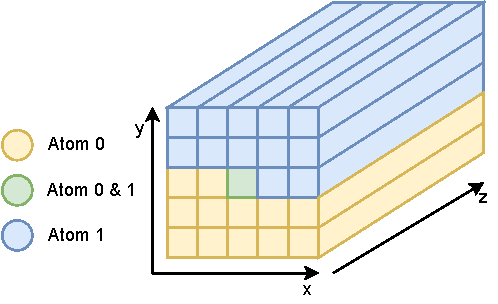
\includegraphics{images/Datenaufteilung_Iteration_2.pdf}
	\caption{Aufteilung des Datenblocks}
	\label{fig:datenaufteilung}
\end{figure}
\begin{figure}
	\center
	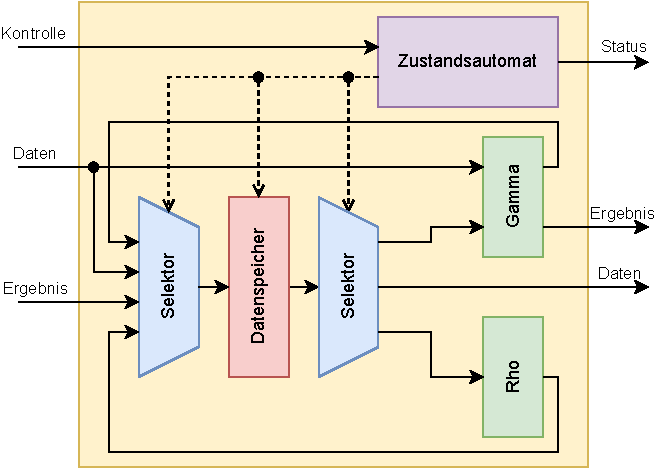
\includegraphics{images/Iteration_2.pdf}
	\caption{Atomaufbau des zweiten Entwurfs}
	\label{fig:aufbau_iteration_2}
\end{figure}

Der Beschleuniger ist in zwei Atome aufgeteilt (Abb. \ref{fig:aufbau_iteration_2}), die jeweils einen Teil des Datenblocks speichern. Beide Atome sind gleich aufgebaut, erst über ein Bit im Kontrollvektor,
den sogenannten \textbf{Atom-Index}, wird festgelegt als welcher Teil des Beschleunigers ein Atom arbeitet. Die Daten sind dabei spaltenorthogonal aufgeteilt, sodass die Lanes 0 bis 12 in Atom 0,
und die Lanes 12 bis 24 in Atom 1 gespeichert werden (Abb. \ref{fig:datenaufteilung}). Die Lane 12 wird dabei absichtlich doppelt gespeichert,
damit beide Atome 13 Lanes speichern, wodurch der gleiche Aufgebaut ermöglicht wird. Jedes Atom speichert somit 13 Lanes aus jeweils 64 Bits, also insgesamt 832 Bits.
Diese Daten werden in einem Block aus FFs gehalten. Über einen Selektor werden aus diesem Datenspeicher die Daten für die Berechnungsblöcke Rho und Gamma sowie für die Kommunikation ausgewählt.
Die Ergebnisse der Berechnungsblöcke sowie die empfangenen Daten werden über einen weiteren Selektor zusammengefügt und wieder im Datenspeicher gespeichert.
Welche Daten von den Selektoren ausgewählt werden und welche im Speicher übernommen werden, bestimmt ein Zustandsautomat. Dieser wird über einen Kontrollvektor von außen gesteuert
und koordiniert die einzelnen Berechnungsschritte und sorgt dafür, dass das Kommunikationsprotokoll befolgt wird.

\subsection{Ablauf einer Berechnung}
\subsubsection{Dateneingabe}
Über den Datenbus werden die Atome mit den Eingabedaten versorgt. Die Eingabe wird entsprechend mit den bereits gespeicherten über ein XOR kombiniert.
Auf diese Weise können der Schwammkonstruktion entsprechend neue Datenblöcke direkt in den Atomen aufgenommen werden ohne,
dass das Ergebis der vorherigen Berechnung erst gelesen werden muss.
\subsubsection{Rho}
Für die Berechnung von Rho werden alle Lanes in einem Atom gleichzeitig in einem Takt wie in einem Schieberegister entsprechend rotiert.
\subsubsection{Gamma}
Die Berechnung von Gamma wird in mehrere Teilschritte aufgeteilt. Atom 0 ist dabei für die Berechnung der Slices 0 bis 31 zuständig und Atom 1
führt die Berechnung für die Slices 32 bis 63 durch. Damit ein neuer Slice berechnet werden kann, muss der vollständige Slice im Atom vorliegen.
Da jeweils 13 Bit schon im eigenen Datenspeicher vorhanden sind, müssen noch 12 Bits aus dem Speicher des anderen Atoms übertragen werden.
Nach der Berechnung muss das Ergebnis in beiden Atomen übernommen werden. Dafür müssen wieder 13 Bits pro Slice übertragen werden.
Um das Kommunikationsprotokoll so einfach wie möglich zu halten und die Ausführungszeit zu minimieren, wird die Berechnung ge-pipelined.
Der 64 Bit breite Voll-Duplex-Kanal zwischen den Atomen wird aufgeteilt in einen 32 Bit breiten Datenkanal und einen 32 Bit breiten Ergebniskanal.
Der genaue Berechnungsverlauf ist noch einmal im Schaubild [Bild Nr] erklärt.
[Schaubild]
\begin{enumerate}
\item Die Daten für Atom 1 werden aus dem Datenspeicher gelesen und an den Datenkanal angelegt.
\item Die Daten für Atom 1 befinden sich im Register des Datenkanals
\item Die Daten für Atom 1 sind am Atom eingetroffen. Gleichzeitig treffen auch die von Atom 1 gesendeten Daten an Atom 0 ein.
Die erhaltenen Daten werden mit den Daten aus dem Speicher von Atom 0 zu vollständigen Slices kombiniert und der Berechnungseinheit bereitgestellt.
\item Die Berechnungseinheit berechnet das Ergebnis und gibt es zurück.
\item Das Ergebnis wird im Datenspeicher übernommen und die Hälfte, die in Atom 1 gespeichert werden soll, wird am Ergebniskanal angelegt.
\item Das Erbebnis im Ergebnisbus befinden sich im Register des Ergebniskanals
\item Das Ergebnis trifft in Atom 1 ein. Gleichzeitig trifft auch das Ergebnis von Atom 1 in Atom 0 ein.
Das erhaltene Ergebnis wird im Datenspeicher übernommen.
\end{enumerate}
Die maximale Anzahl an Slices, die gleichzeitig in einem Atom berechnet werden kann, ergibt sich in diesem Fall aus der stark beschränkten Bandbreite
des Kommunikationskanals. In dem 32 Bit breiten Kanal können maximal zwei 12 Bit bzw 13 Bit Einträge in einem Takt übertragen werden.
Um den gesammten Blockteil zu berechnen, muss die oben aufgeführte Berechnungsabfolge also 16 Mal mit jeweils 2 Slices durchgeführt werden.
Da die Berechnung der 7 Schritte in einer Pipeline durchgeführt wird, beträgt die Berechnungsdauer nicht 16 * 7 = 112 Schritte,
sondern nur 7 + (16 - 1) = 22 Schritte.

\subsection{Bewertung}
Die Ausführungszeit für eine Iteration der modifizierten Rundenfunktion ist wie erwartet etwa um einen Faktor 30 langsamer als die Implementierung der ersten Iteration.
Dies ist wie bereits erklärt hauptsächlich der Aufteilung der Gamma-Funktion in 16 Teilschritte geschuldet, sowie der damit einhergehenden Verzögerung.
Anders jedoch als erwartet, ist die Größe der Atome durch das Aufteilen der Berechnung und des Datenspeichers nicht wie gewünscht gesunken.
Tatsächlich ist der Entwurf mit seinen etwa 4600 LUTs nochmal um gut 37\% größer. Dafür gibt es zwei wesentliche Gründe: den Zustandsautomaten sowie die Speicherkomplexität,
die in der Überlegung für das Design nicht bedacht wurden.
\subsubsection{Zustandsautomat}
Der Zustandsautomat besteht aus einem Iterator, der in jedem Takt hochgezählt wird und anhand dessen die Steuersignale für die anderen Komponenten genertiert werden.
Entgegen der ursprünglichen Annahme, dass seine Größe aufgrund der Einfachheit der Aufgabe vernachlässigbar ist, nimmt er in diesem Design etwa 300 LUTs ein.
Auch wenn sich die konkrete Implementierung noch optimieren lässt, so ist klar geworden, dass die weitere Erhöhung der Berechnungskomplexität mit Bedacht durchgeführt werden muss,
da der Zustandsautomat dadurch nur noch größer wird.
\subsubsection{Schreib- und Lesemuster}
Im ersten Entwurf wird der Wert jedes Bits im Register entweder von der Eingabe oder von der Ausgabe der Rundenfunktion bestimmt.
Im zweiten Entwurf hingegen hängt dieser Wert ab von der Eingabe, des Ergebnisses der Rho-Rotation sowie einem Bit im Ergebnis-Kanal.
Welches Bit aus dem Ergebniskanal für ein Bit im Datenspeicher bestimmt ist, legt der Zustandsautomat und auch der Atom-Index fest.
Diese Auswahlschaltung sowie die Entscheidung, wann genau das Bit im Register überschrieben werden muss (im ersten Entwurf wurden einfach alle Bits in jedem Takt überschrieben, wenn das Kontrollsignal aktiv war),
benötigen schon mehr Platz als die Reduktion der Datenmenge einspart.
Analog ist auch das Lesen der Daten komplizierter geworden. Die Gamma-Funktion sowie der Datenkanal müssen anhand des Zustandsautomaten und des Atom-Indexes aus allen Bits nur ein par auswählen.
\subsubsection{Gamma-Funktion}
Die Gamma-Funktion übernimmt bis auf Rho alle Subfunktionen der Standard-Rundenfunktion. Da die Berechnung auf zwei Atome aufgeteilt ist und auch nicht alle Slices in einem Atom gleichzeitig berechnet werden,
ist die Komplexität der Gamma-Funktion sehr stark geschrumpft, sodass das aktuelle Design nur etwa 70 LUTs benötigt. Eine weitere Optimierung der Gamma-Funktion ist daher auch in weiteren Iterationen nicht mehr nötig.

\subsection{Optimierungsansätze}
Die starke Steigerung der Speicherkomplexität ist das Hauptproblem des Entwurfs und weitere Verbesserungen müssen hier ansetzen, um den Beschleuniger aus die erforderliche Größe reduzieren zu können.
Um die Speicherverwaltung vollständig aus dem Design zu entfernen, hatten wir die Nutzung der BRAM-Blöcke in den Überlegungen des ersten Entwurfs schon einmal erwähnt und uns letztendlich dagegen entschieden,
weil das Festlegen auf einen Tile-orientierten Speicher bedeutet, dass die Rho-Funktion, die eigentlich auf Lanes arbeitet, so implementiert werden muss, dass sie mit Tiles arbeiten kann.
\subsubsection{Transformation der Rho-Funktion}


\subsubsection{BRAM als Datenspeicher}


\chapter{Ergebnisse}

\chapter{Fazit}

\chapter{Template Stuff that is still here}

\section{Some Template Comments}
\label{sec:comments}

\begin{outline}
  \1 It is recommended to use one sentence per line of the latex source code.
  That is a good compromise between (i) `diffs' when using repositories, and (ii) forward-/backward search between latex source code and pdf output.
  \1 Note that you can have multiple refs in the same \textbackslash cref block (e.g., \cref{sec:motivation,sec:comments,sec:statement,sec:results,fig:popcount}), but there must not be spaces after the commas.
  \1 Note that you should use \textbackslash Cref (upper-case C) at the beginning of a sentence and \textbackslash cref (lower-case c) in the middle of a sentence.
  They are defined differently, such that the upper-case C version does not use abbreviations (which is recommended for the beginning of a sentence), e.g., \cref{eq:node} vs. \Cref{eq:node}.
  \1 You can use the outline environment to collect itemized points before actually writing your text.
    \2 It helps structuring your ideas by simplifying indentation of items
    \3 Like here.
\end{outline}


\section{Problem Statement}
\label{sec:statement}

Based on a partitioning $P \subset 2^V$, i.e., $p_i, p_j \in P, p_i \ne p_j \Rightarrow p_i \cap p_j = \emptyset, \bigcup\limits_P = V$, an equivalence relation $\sim_P$ as well as the partition graph $G_P$ are defined as follows:
\begin{align}
  \sim_P &= \{(v_1,v_2) \in V | \exists p \in P: v_1\in p \wedge v_2 \in p\}\\
  G_P &= (V_P, E_P) = (V/\sim_P, \{ ([v_1]_{\sim_P}, [v_2]_{\sim_P}) |\: (v_1,v_2) \in E \})
  \label{eq:node}
\end{align}



\section{Results}
\label{sec:results}

Following is the discussion of obtained results.

\begin{figure}[ht]
  \center
  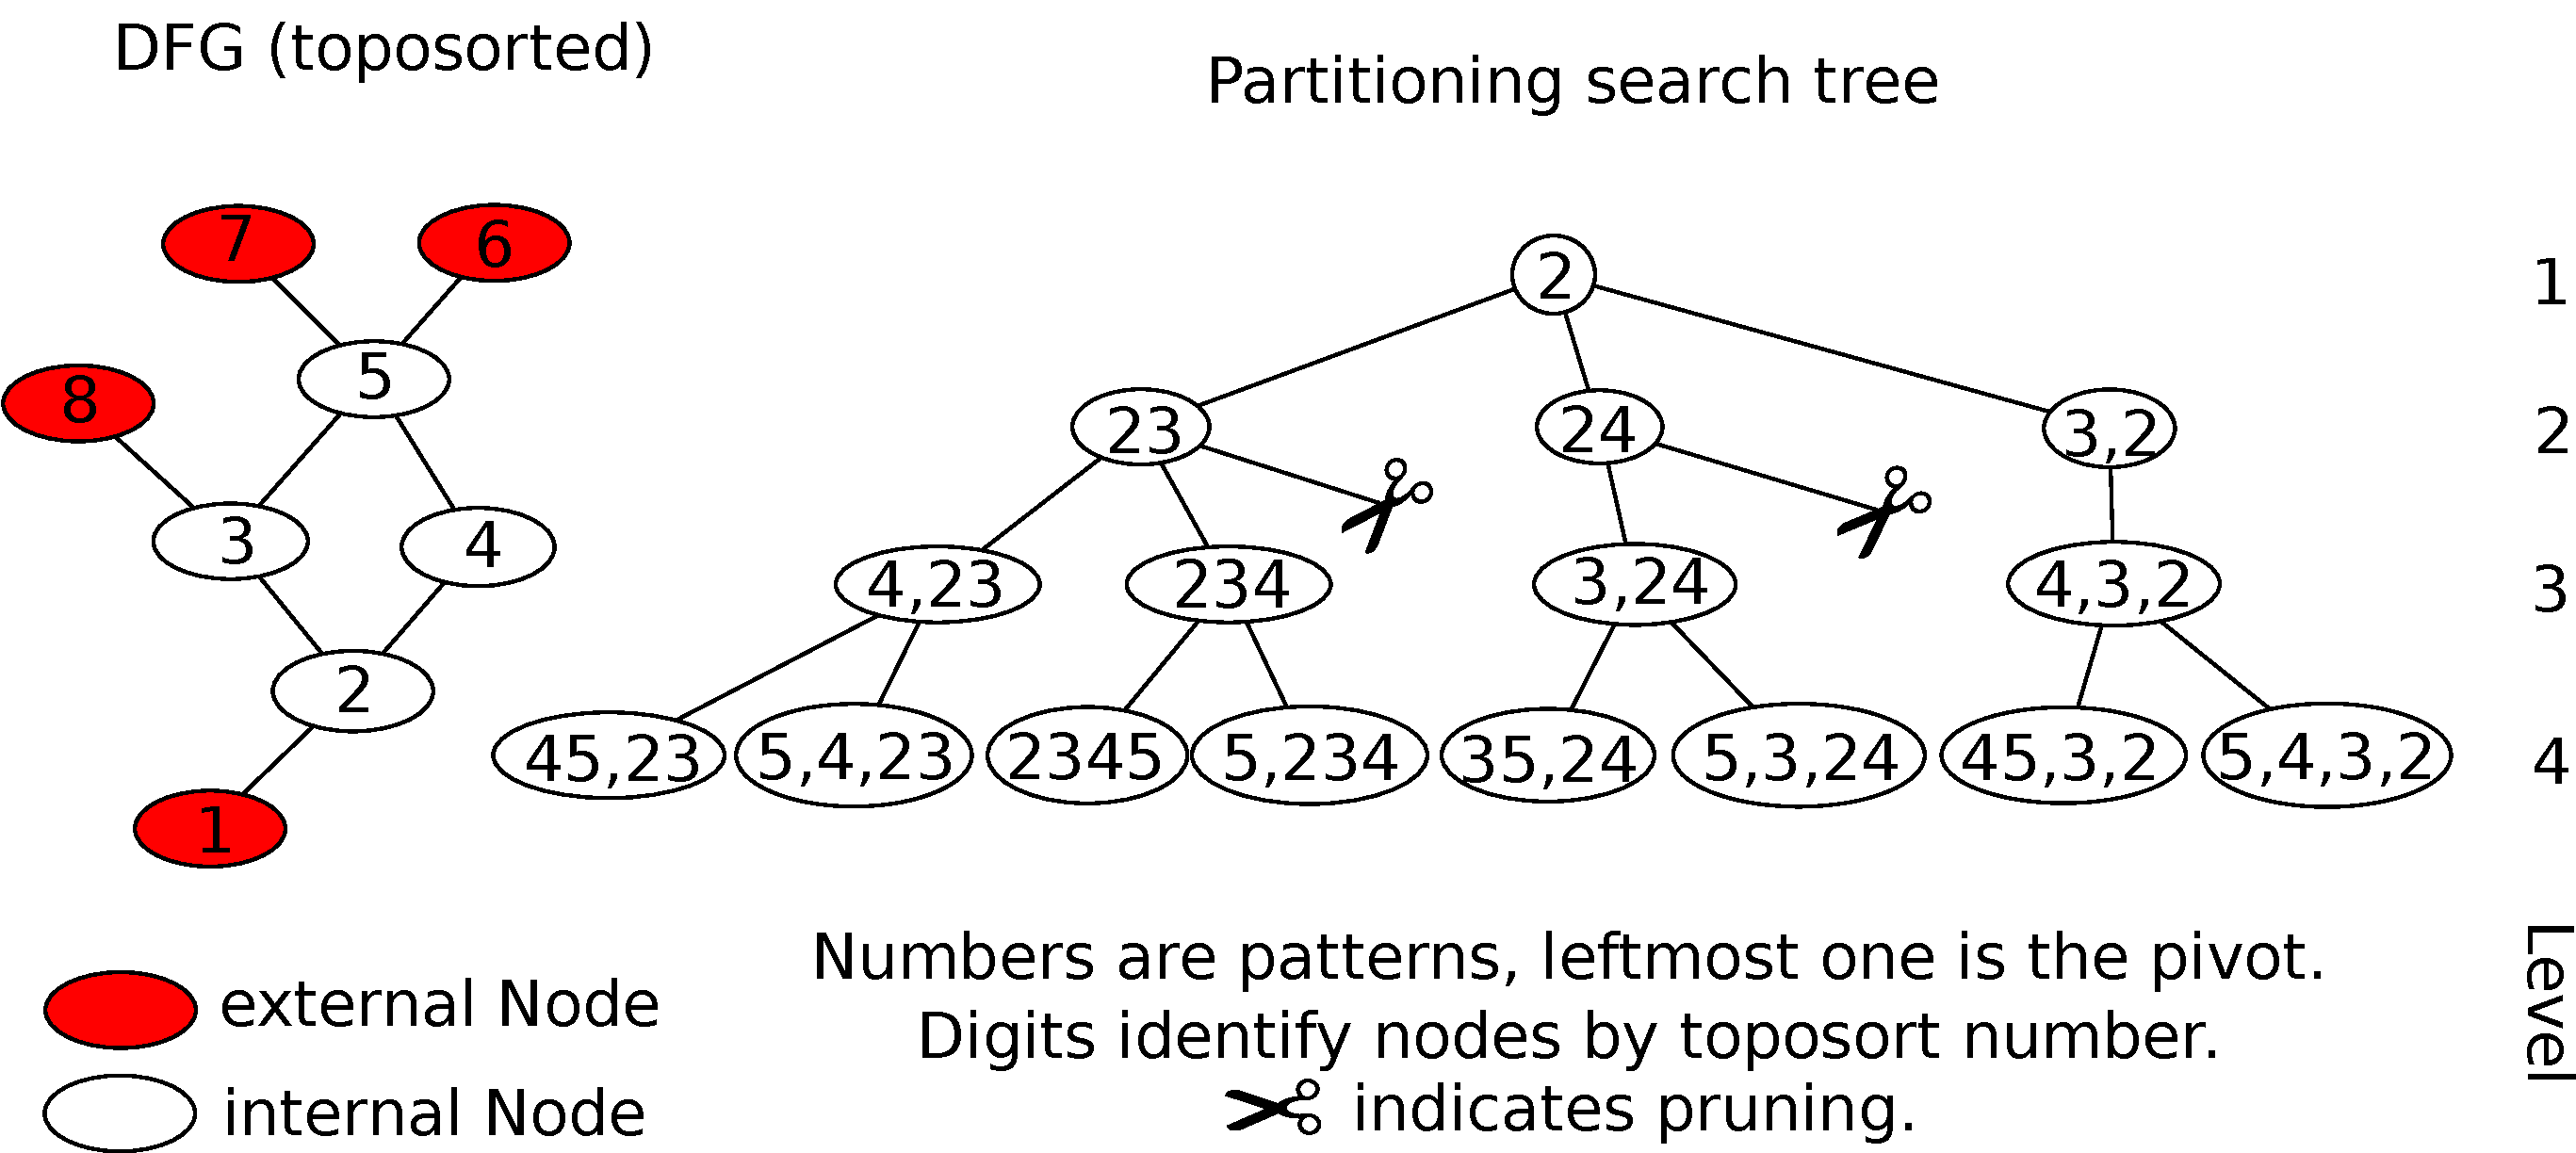
\includegraphics[scale=0.33]{searchtree.pdf}
  \caption{Topologically sorted DFG along with the complete search tree of the partition enumeration algorithm.}
  \label{fig:searchtree}
\end{figure}



\begin{table}
  \centering
  \begin{tabular}{lrrrr}
                &   types  &      types  &   atoms  &      atoms  \\
    SI          &  manual  &  generated  &  manual  &  generated  \\
    \hline
    htfour      &       1  &          4  &       8  &         81  \\
    satdfour    &       3  &          8  &      16  &        104  \\
    dctfour     &       2  &          9  &      12  &         90  \\
    sadsixteen  &       1  &          4  &      64  &        255  \\
  \end{tabular}
  \caption{Comparison of generated SI graphs vs. hand-crafted ones.}
  \label{tab:manualeval}
\end{table}


\begin{figure}
\lstset{language=C}
\begin{lstlisting}[label={lst:popcount}]
uint32_t popcount_a(uint32_t x)
{
  x -= ((x >> 1) & 0x55555555);
  x = (x & 0x33333333) + ((x >> 2) & 0x33333333);
  x = (x + (x >> 4)) & 0x0f0f0f0f;
  x += x >> 8;
  x += x >> 16;
  return x & 0x3f;
}
\end{lstlisting}
\caption{C-Code from \cite{warren2003hacker} to compute the number of set bits of a 32-bit value.}
\label{fig:popcount}
\end{figure}

